% ==============================================================================
% Instituto Federal de Alagoas
% Modelo usado para Trabalho De Conclusão de Curso (TCC) da Coordenação de 
% Informática do IFAL - Campus Maceió
%
% Autor:  Leonardo Melo de Medeiros
% Endereço: https://www.overleaf.com/read/swrgmkkmhwzs
% Baseado no modelo do IFRN feito pelo Prof. Rodrigo Siqueira
% ==============================================================================

% Classe .......................................................................
\documentclass[a4paper,12pt,openany,oneside]{book}

%ATENÇÃO USAR PADRÃO DE CONDIFICAÇÃO DO LINUX UTF8
%PARA SABER SE VC O ESTÁ USANDO BASTA PERCEBER A ACENTUAÇÃO ERRADA
\usepackage[utf8]{inputenc}

%Para adicionar figuras
\usepackage{graphicx}

%Para usar Times new Roman
\usepackage{pslatex}



% Pacotes ....................................................................................
% Pacotes Principais -----------------------------------------------------------
\usepackage[portuges,brazil]{babel}
\usepackage{ae} 

%Linux ou Windows com UTF8
\usepackage[utf8]{inputenc}

%\usepackage[latin1]{inputenc}

%NO MAC ao inv�s de latin1 deve-se usar o applemac
%\usepackage[applemac]{inputenc}


% Formatacaoo de capitulos ------------------------------------------------------
%\usepackage{capitulos}

% Figuras e Imagens ------------------------------------------------------------
\usepackage{graphicx}
% Figuras lado a lado
%\usepackage{epsfig} - REMOVIDO
%\usepackage{subfigure} - REMOVIDO

% Para poder ter tabelas com colunas de largura auto-ajust�vel
\usepackage{tabularx}

% Utilizar H para inserir as imagens REALMENTE onde eu desejo
%\usepackage{float} - REMOVIDO

% Para que os primeiros par�grafos das se��es tamb�m sejam indentados
% \usepackage{indentfirst} - REMOVIDO

%Permitir usar o comando \citeasnoun que coloca o nome na cita?�o
\usepackage{harvard}


% Fontes -----------------------------------------------------------------------
%\usepackage[T1]{fontenc} - REMOVIDO
%\usepackage{pslatex} - REMOVIDO

% Matem�tico -------------------------------------------------------------------
%\usepackage{amsmath} - REMOVIDO
%\usepackage{amstext} - REMOVIDO

% Simbolos ---------------------------------------------------------------------
%\usepackage{textcomp} - REMOVIDO

% Tabelas ----------------------------------------------------------------------
%\usepackage{multirow} - REMOVIDO
% Colorir a tabela
%\usepackage{colortbl} - REMOVIDO

% Gloss�rio --------------------------------------------------------------------
%\usepackage[portuguese,noprefix]{nomencl}
%\usepackage{makeglo}

% Outros pacotes ---------------------------------------------------------------
%\usepackage{noitemsep} - REMOVIDO

%Subsubsection
%\usepackage{chngcntr} - REMOVIDO

% Para permitir espa�amento simples, 1 1/2 e duplo
\usepackage{setspace}

% Para executar um comando depois do fim da p�gina corrente
%\usepackage{afterpage} - REMOVIDO

% Para poder incluir arquivos Postscript com cores (do Xfig, por exemplo)
%\usepackage{color} - REMOVIDO

  % Itens numerados
%\usepackage{enumerate} - REMOVIDO

% Coment�rios em bloco
%\usepackage{verbatim} - REMOVIDO

% Refer�ncias ------------------------------------------------------------------
%\usepackage{html} - REMOVIDO
%\usepackage{url} - REMOVIDO
%\usepackage[abbr]{harvard}	% As chamadas s�o sempre abreviadas - REMOVIDO
%\harvardparenthesis{square}	% Colchetes nas chamadas - REMOVIDO
%\harvardyearparenthesis{round}	% Par�ntesis nos anos das refer�ncias - REMOVIDO
%\renewcommand{\harvardand}{e}	% Substituir "&" por "e" nas refer�ncias
%\renewcommand{\harvardurl}{URL: \url} - REMOVIDO

% Novos Comandos .....................................................................
% newcommand define novos comandos, que podem passar a ser usados da
% mesma forma que os comandos LaTeX de base.

% Configura��o da fonte
%\renewcommand{\familydefault}{\sfdefault}

% Margens ----------------------------------------------------------------------
%\setlength{\oddsidemargin}{3.5cm}
%\setlength{\evensidemargin}{2.5cm}
%\setlength{\textwidth}{15cm}
%\addtolength{\oddsidemargin}{-1in}
%\addtolength{\evensidemargin}{-1in}
%%
%\setlength{\topmargin}{2.0cm}
%\setlength{\headheight}{1.0cm}
%\setlength{\headsep}{1.0cm}
%\setlength{\textheight}{22.7cm}
%\setlength{\footskip}{1.0cm}
%\addtolength{\topmargin}{-1in}

% Cap�tulos --------------------------------------------------------------------
% N�o aparecer o n�mero na primeira p�gina dos cap�tulos
\newcommand{\mychapter}[1]{\chapter{#1}\thispagestyle{empty}}
\newcommand{\mychapterstar}[1]{\chapter*{#1}\thispagestyle{empty}}

% Os cap�tulos sem n�mero
%\newcommand{\mychapterast}[1]{\chapter*{#1}\thispagestyle{empty}
%\chaptermark{#1}
%\afterpage{\markboth{\uppercase{#1}}{\rightmark}}
%\markboth{\uppercase{#1}}{}
%}

%Referencias
%\newcommand{\BibTeX}{\textsc{B\hspace{-0.1em}i\hspace{-0.1em}b\hspace{-0.3em}}\TeX}

% Comandos matem�ticos ---------------------------------------------------------
% Implica��o em f�rmulas
%\newcommand{\implica}{\quad\Rightarrow\quad} %Meio de linha
%\newcommand{\implicafim}{\quad\Rightarrow}   %Fim de linha
%\newcommand{\tende}{\rightarrow}

% Fra��o com parenteses
%\newcommand{\pfrac}[2]{\parent{\frac{#1}{#2}}}

% Transformada de Laplace e transformada Z
%\newcommand{\lapl}{\pounds}
%\newcommand{\transfz}{\mathcal{Z}}

% Sequ�ncias
%\newcommand{\sequencia}[4]{$#1_{#2}$, $#1_{#3}$, \ldots, $#1_{#4}$}

% Se��es sem n�mero
%\newcommand{\mysectionast}[1]{\section*{#1}
%\addcontentsline{toc}{section}{#1}
%\markright{\uppercase{#1}}
%}

% No tabularx, as celulas devem ser centradas verticalmente
\renewcommand{\tabularxcolumn}[1]{m{#1}}

% C�lulas centralizadas horizontalmente no tabularx
\newcolumntype{C}{>{\centering\arraybackslash}X}


% Outros ----------------------------------------------------------------------
%\newcommand{\chave}[1]{\left\{#1\right\}}
%\newcommand{\colchete}[1]{\left[#1\right]}
%\newcommand{\parent}[1]{\left(#1\right)}

%%subsubsection
%\newcounter{subcount}
%\newenvironment{mysub}
%{\begin{list}
%{\textbf{\thesubsubsection.\arabic{subcount}}}
%{\setlength{\itemindent}{2.2em}
%\setlength{\rightmargin}{.6in}
%\setlength{\labelwidth}{1in}
%\setlength{\labelsep}{.2in}
%\setlength{\parsep}{.5ex plus .2ex minus .1ex}
%\setlength{\itemsep}{0ex plus .2ex minus 0ex}
%\usecounter{subcount}}
%}


%\citationmode{abbr}

% Inicia o texto
\begin{document}

% Paginas iniciais (sem numeração)
\pagestyle{empty}

% P?gina de rosto (capa interna)
%
% ********** Página de Rosto
%

% titlepage gera páginas sem numeração
\begin{titlepage}

\begin{center}

\large
\textbf{Instituto Federal de Alagoas\\
 Campus Maceió\\
 Bacharelado em Sistemas de Informação}
\end{center}

\begin{center}
\vfill
\vfill
\vfill
\Large

\textbf{Nome do Aluno} \\
%\textbf{Autor 2}


% O vfill é um espaço vertical que assume a máxima dimensão possível
% Os vfill's desta página foram utilizados para que o texto ocupe
% toda a folha
\vfill

\LARGE

\textbf{Título do TCC}

\vfill


\vfill

\vfill

\vfill

\vfill

\vfill

\vfill

\vfill

\vfill

\large

%\hfill
%\parbox{0.5\linewidth}{\textbf{Trabalho de Conclusão de Curso apresentado ao Curso de Bacharelado em Sistemas de Informação do Instituto Federal de Alagoas como requisito parcial para obtenção do título de bacharel em Sistemas de Informação.}
%
%
%\vfill
%
%\large

%Data
Maceió, ano

\end{center}

\end{titlepage}
  

% P?gina de rosto (capa interna)
%
% ********** Página de Rosto
%

% titlepage gera páginas sem numeração
\begin{titlepage}

\begin{center}

\small

% O comando @{} no ambiente tabular x é para criar um novo delimitador
% entre colunas que não a barra vertical | que é normalmente utilizada.
% O delimitador desejado vai entre as chaves. No exemplo, não há nada,
% de modo que o delimitador é vazio. Este recurso está sendo usado para
% eliminar o espaço que geralmente existe entre as colunas
\begin{tabularx}{\linewidth}{ c X }
% A figura foi colocada dentro de um parbox para que fique verticalmente
% centralizada em relação ao resto da linha
\parbox[c]{3cm}{\includegraphics[width=\linewidth]{IFRN}} &
\begin{center}
\textsf{\textsc{Instituto Federal de Alagoas\\
 Campus Maceió\\
 Coordenação de Informática \\
 Curso Superior de Bacharelado em Sistemas de Informação
}} 
\end{center}

\end{tabularx}


% O vfill é um espaço vertical que assume a máxima dimensão possível
% Os vfill's desta página foram utilizados para que o texto ocupe
% toda a folha
\vfill

\LARGE

\textbf{Título do Trabalho}

\vfill

\Large

\textbf{Autor 1} \\
%\textbf{Autor 2}

\vfill

\normalsize
Orientador por:\\
Prof. Dr. Leonardo Melo de Medeiros\\
%Prof. Co-orientaddor


\vfill

\hfill
\parbox{0.5\linewidth}{Trabalho de Conclusão de Curso apresentado como requisito para obtenção do título de Bacharel em Sistemas de Informação.}


\vfill

\large

%\hfill
%\parbox{0.5\linewidth}{\textbf{Trabalho de Conclusão de Curso apresentado ao Curso de Bacharelado em Sistemas de Informação do Instituto Federal de Alagoas como requisito parcial para obtenção do título de bacharel em Sistemas de Informação.}
%
%
%\vfill
%
%\large

%Data
Maceió, AL, agosto de 2016

\end{center}

\end{titlepage}
  

%Espa?amento 1 1/2
\onehalfspacing  

% Paginas introdut?rias (com numeração romana)
\frontmatter


% Lista de figuras (gerada automaticamente)
\cleardoublepage 
\addcontentsline{toc}{chapter}{Lista de Figuras}  
\listoffigures  



% Lista de tabelas (gerada automaticamente)
\cleardoublepage 
\addcontentsline{toc}{chapter}{Lista de Tabelas}   
\listoftables

\cleardoublepage 
\addcontentsline{toc}{chapter}{Lista de Símbolos}  
\ListadeSimbolos
\begin{acronym}
	\acro{dp}[Parkinson]{Doença de Parkinson}
	\acro{svm} [SVM]{Máquina de Vetor de Suporte}
\end{acronym}


% Lista de conteúdo (sumário, gerado automaticamente)
\addcontentsline{toc}{chapter}{Sumário}   
\tableofcontents  


  

% P?ginas do texto principal (com cabe?alho)
\mainmatter
\pagestyle{headings}

% Para facilitar a organização, foi criado um diretório para cada
% capítulo do documento, pois assim os arquivos das figuras ficam
% classificados por cap?tulos

% Introdução
%%
%% Capítulo 1: Modelo de Capítulo
%%

% Está sendo usando o comando \mychapter, que foi definido no arquivo
% comandos.tex. Este comando \mychapter é essencialmente o mesmo que o
% comando \chapter, com a diferença que acrescenta um \thispagestyle{empty}
% após o \chapter. Isto é necessário para corrigir um erro de LaTeX, que
% coloca um número de página no rodapé de todas as páginas iniciais dos
% capítulos, mesmo quando o estilo de numeração escolhido é outro.
\mychapter{Introdução}
\label{Cap:introducao}

%O que escrever
A introdução deverá ser escrita depois do desenvolvimento do trabalho. Nela deve conter a explicação do que será abordado no trabalho e se necessário um histórico da necessidade do conteúdo. Aqui é importante colocar citação direta onde se pode dizer que Segundo \citeasnoun{Bernardete} e ainda escrever seu próprio texto através da leitura de outros trabalhos e fazer uma citação indireta \cite{Bernardete}. Não é muito interessante colocar figuras aqui na introdução embora não seja proibido. Procure escrever de forma resumida, mas faça valer ao leitor o que de importante ele encontrará na leitura, ou seja, aqui deve-se "vender o peixe" do trabalho.





%Sobre esse trabalho
Descreva o máximo do que se trata o trabalho e sua importância.

\section{Motivação}
\label{Sec:Motivacao}
%Motivação
Explique aqui porque iniciou as pesquisas no tema e qual a motivação de desenvolver esse trabalho.

\section{Objetivo}
\label{Sec:Objetivo}
%Objetivo
Descreva o objetivo principal do trabalho. Tente criar um parágrafo resumindo o que seu trabalho fará. Depois seja mais específico, pode inclusive criar tópicos para a Seção \ref{Sec:ObjetivoEspecifico}.

\subsection{Objetivo específico}
\label{Sec:ObjetivoEspecifico}
\begin{itemize}
  \item Criar uma ferramenta que ... ;
  \item Criar ... ;
\end{itemize}



\section{Organização do trabalho}
\label{Sec:Organização}
%Organiza�‹o do trabalho   
Sempre que precisar referenciar outra parte de seu trabalho use o comando \\ref apontando para o que você colocou no \\label como por exemplo essa Seção \ref{Sec:Organização}. Aqui você deverá informar como e porque seu trabalho foi organizado, informando o que será abordado em cada capítulo.


 

% Desenvolvimento
%%
%% Capítulo 2: Desenvolvimento do trabalho
%%

\mychapter{Desenvolvimento}
\label{Cap:desenvolvimento}

Este capítulo apresenta considerações de ordem geral sobre a
organização e desenvolvimento do texto.

\section{O que escrever}
\label{Sec:oque}

É possível iniciar o capítulo de desenvolvimento informando como será desenvolvido o trabalho e o detalhe das ferramentas ou o conteúdo que será abordado e utilizado. Em seguida comente o conteúdo em conjunto com o conhecimento adquirido junto as consultas e referências bibliográficas. 
Isso demonstra que foi feito uma pesquisa anterior e mostra que o trabalho tem relevância científica, ou seja, não está sendo "inventada a roda". 




Exemplo:


A partir desse método de separação dos dados, é que a~\ac{svm} foi aplicada para classificar indivíduos diagnosticados com~\ac{dp} ante indivíduos sem o diagnóstico estabelecido. Para corroborar com a nossa escolha de SVM, encontrou-se trabalhos de classificação de indivíduos com parkinson utilizando a mesma abordagem~\cite{bradmonitor2015,svmparkinson2010,patel_monitoring_2009}. No entanto, o que diferencia este trabalho dos demais, é que os dados classificados foram adquiridos utilizando a abordagem de um jogo eletrônico que induz o paciente a executar movimentos para a avaliação motora~\cite{quantitativeparkinson2011,wiiassesspark2016}. 




\section{Divisões do documento e referências cruzadas}
\label{Sec:divisoes}

Sempre que for modificar/aprofundar partes de um tema, é interessante criar uma seção de maneira a tornar o assunto mais focado e facilitar a leitura. 
Não crie seções sem que estas tenham nenhum texto ou sigam direto para outra seção. Se isso acontecer é melhor rever como está organizado o texto pois pode se tornar necessário remover capítulos ou seções. 

No final de cada capítulo é importante apresentar comentário do que foi desenvolvido no texto permitindo ao leitor compreender a visão geral do conteúdo e pode-se inclusive contextualizar o capítulo seguinte.



\mychapter{Figuras, tabelas e gráficos}
\label{Cap:figuras}

Uma das maiores dificuldades na edição de textos de qualidade é o
posicionamento dos elementos gráficos: figuras, gráficos e
tabelas. Como estes elementos muitas vezes são grandes, aparece o
dilema sobre o que fazer quando uma quebra de página deveria acontecer
no meio do elemento. Há duas possibilidades:
\begin{enumerate}
\item O autor informa exatamente onde o elemento gr‡fico deve ficar no
texto, evitando que quebras de páginas aconteçam no meio de um
elemento. O problema com esta abordagem é que todo o trabalho de
posicionamento pode ser perdido caso se inclua ou se exclua algum
texto ou elemento.
\item O editor de texto posiciona os elementos gráficos de forma a não
deixar espaços em branco nas páginas. Estes elementos que podem ser
posicionados pelo editor são conhecidos como \emph{elementos
flutuantes}. O problema com esta abordagem é que o posicionamento
adotado pode não corresponder às expectativas do autor.
\end{enumerate}



\section{Tabelas em \LaTeX}
\label{Sec:tabelas}

Tabelas são construpídas com comandos próprios do \LaTeX, notadamente o
ambiente \texttt{tabular}. Nada obriga a que o ambiente
\texttt{tabular} esteja sempre posicionado em um elemento
flutuante. Se você quiser impor que uma tabela fique obrigatoriamente
em uma determinada posição do texto, basta não colocar o
\texttt{tabular} dentro de um \texttt{table}. Tabelas podem até ser
incluídas no meio de uma frase.  Por exemplo, eu posso dizer que se um
jogo da velha está na configuração \textsf{\tiny\begin{tabular}{c|c|c}
x & & x \\ \hline & & o \\ \hline x & o & \end{tabular}} e se o
jogador ``\textsf{x}'' sabe jogar, ent‹o o jogador ``\textsf{o}'' irá
perder, independentemente da jogada que faça.

 Exemplos de
colunas com diferentes larguras e alinhamentos podem ser vistos na
tabela \ref{Tab:larguracolunas}.

\begin{table}[htbp]
\begin{tabularx}{\linewidth}{|p{3cm}|X|l|} \hline
COLUNA p & COLUNA X & COLUNA l \\ \hline
Largura fixa (não depende do conteúdo) &
Expandível &
Ajustável \\ \hline
Alinhada no topo &
Alinhada à esquerda &
Alinhada à esquerda \\ \hline
\end{tabularx}
\\[0.5cm]
\begin{tabularx}{\linewidth}{|b{3cm}|C|r|} \hline
COLUNA b & COLUNA C (ver \texttt{comandos.tex}) & COLUNA r \\ \hline
Largura fixa (não depende do conteúdo) &
Expandível &
Ajustável \\ \hline
Alinhada na base &
Centralizada &
Alinhada à direita \\ \hline
\end{tabularx} 
\caption{Tabelas com colunas de diferentes larguras e alinhamentos}
\label{Tab:larguracolunas}
\end{table}





\section{Figuras em \LaTeX}
\label{Sec:figuras}

As figuras (imagens, desenhos, gr‡ficos, etc.) devem ser produzidas
por ferramentas externas ao \LaTeX, salvas em um arquivo e inseridas
no texto usando o comando \texttt{includegraphics}. Da mesma forma
que as tabelas, as figuras podem ser flutuantes, caso sejam
inseridas dentro de um ambiente \texttt{figure}, ou ter uma posição
fixa no texto (como aqui: 
\includegraphics{figuras/eu}).

O formato em que você deve salvar os arquivos das figuras para que
possa incluí-las no texto depende de como você pretende compilar
o código fonte:
\begin{itemize}
\item se o texto vai ser compilado com \texttt{latex}, todos os
arquivos devem estar no formato EPS (\emph{Encapsulated PostScipt});
\item se o texto vai ser compilado com \texttt{pdflatex}, os
arquivos devem estar nos formatos PDF ou JPEG (outros formatos são
aceitos, mas estes são os recomendáveis).
\end{itemize}

A figura \ref{Fig:belmonte} mostra um exemplo de inclusão de uma
imagem EPS no texto \LaTeX.

\begin{figure}[htbp!]
\begin{center}
% fbox faz uma borda ao redor do seu argumento
\fbox{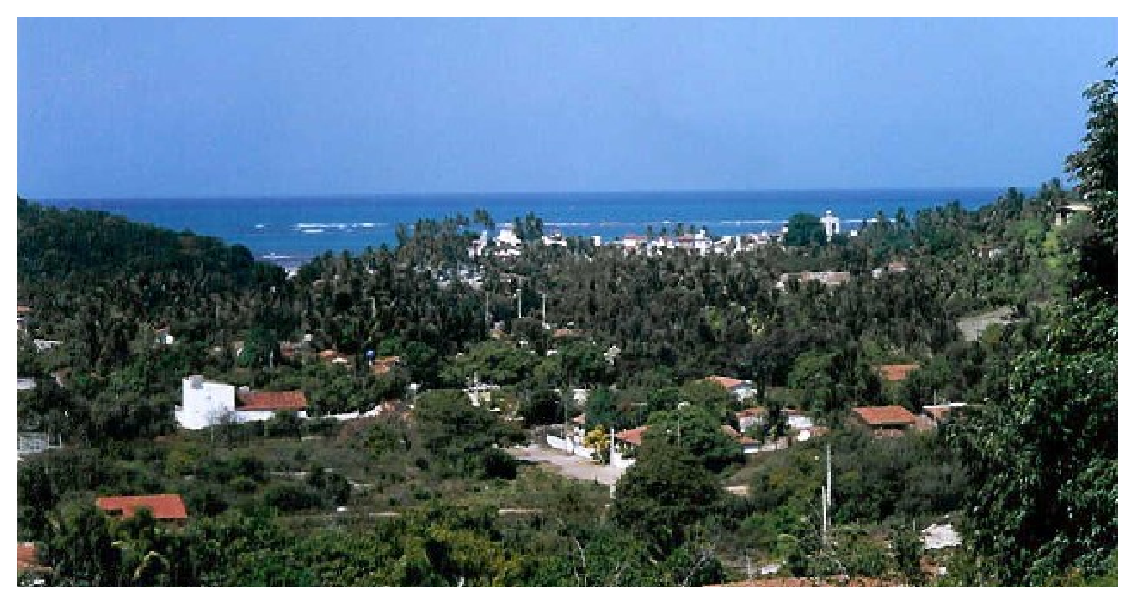
\includegraphics[width=0.75\linewidth]{figuras/belmonte}}
\caption{Exemplo de imagem real}
\label{Fig:belmonte}
\end{center} 
\end{figure}



 

% Conclusões
%%
%% Capítulo 5: Conclusões
%%

\mychapter{Conclusão}
\label{Cap:conclusao}

Neste capítulo terá o fechamento do seu trabalho. Informe como foram os resultados obtidos. Quais seus comentários e conhecimento obtidos a partir das experiências executadas. Evite citar termos com juízo de valor como: "é ruim ...", "é bom ...", etc. prefira colocar: "foi possível observar que 90\% das amostras ...". Aqui também não se deve colocar figuras, tabelas, etc. mas referenciar as que foram abordadas no texto fazendo o fechamento dos resultados.

%TRAB. FUTUROS
\section{Trabalhos Futuros}
\label{Sec:Trabalhos Futuros}
Descreva os trabalhos que você percebeu que daria pra fazer como melhoria, continuidade do que você fez e que por algum motivo não foi possível de fazê-lo.

 

\backmatter


% Referências bibliográficas (geradas automaticamente)
%\bibliographystyle{ppgee}
\bibliographystyle{dcu}
\addcontentsline{toc}{chapter}{Referências bibliográficas}
%Arquivo com as bibliografias
\bibliography{bibliografia}


\end{document}